\documentclass[review,11pt]{elsarticle}
%\documentclass[preprint,review,12pt,authoryear]{elsarticle}
\usepackage{lineno,hyperref,ulem,todonotes}
\usepackage{rotating}
\usepackage{amsmath}
\modulolinenumbers[5]
%\usepackage{natbib}
\usepackage{tabularx,ragged2e,booktabs,caption}
\journal{Computational Geosciences}

%%%%%%%%%%%%%%%%%%%%%%%
%% Elsevier bibliography styles
%%%%%%%%%%%%%%%%%%%%%%%
%% To change the style, put a % in front of the second line of the current style and
%% remove the % from the second line of the style you would like to use.
%%%%%%%%%%%%%%%%%%%%%%%

%% Numbered
\bibliographystyle{model1-num-names}

%% Numbered without titles
%\bibliographystyle{model1a-num-names}

%% Harvard
%\bibliographystyle{model2-names.bst}\biboptions{authoryear}

%% Vancouver numbered
%\usepackage{numcompress}\bibliographystyle{model3-num-names}

%% Vancouver name/year
%\usepackage{numcompress}\bibliographystyle{model4-names}\biboptions{authoryear}

%% APA style
%\bibliographystyle{model5-names}\biboptions{authoryear}

%% AMA style
%\usepackage{numcompress}\bibliographystyle{model6-num-names}

%% `Elsevier LaTeX' style
%\bibliographystyle{elsarticle-num}
%%%%%%%%%%%%%%%%%%%%%%%

\begin{document}

\begin{frontmatter}

\title{Simulation Study of a Novel Subgrid Model for Microtopography Effect on Surface Flow}

%\author[ornl]{Ahmad Jan \corref{cor}} \author[lanl1]{Ethan T. Coon} \author[ornl]{Scott L. Painter} \author[lanl2]{Rao Garimella} \author[lanl2]{J. David Moulton}

%\address[ornl]{Climate Change Science Institute and Environmental Sciences Division, Oak Ridge National Laboratory, Oak Ridge, Tennessee, USA\fnref{copyrightnotice}} 
%\address[lanl1]{Computational Earth Sciences Group, Earth and Environmental Sciences Division, Los Alamos National Laboratory, Los Alamos, New Mexico, USA} 
%\address[lanl2]{Applied Mathematics and Plasma Physics Group, Theoretical Division, Los Alamos National Laboratory, Los Alamos, New Mexico, USA} 


%\cortext[cor]{Corresponding Author: Ahmad Jan; Email: jana@ornl.gov; Phone: (865) 576-8175.}



\begin{abstract}
A subgrid model for accurate representation of surface flow behavior, influenced by surface microtopography, at larger spatial scales is presented.
%This article presents a subgrid model to represent accurate surface flow behavior, influenced by surface microtopography, at large spatial scales. 
It is well understood that the spatial heterogeneity in the surface microtopography serves a critical role in the surface water retention, surface/subsurface interactions, and delay runoff, and thereby significantly affects the shape of the hydrographs. But high-resolution simulations at large spatial and temporal scales are not tractable. Watershed-scale simulations demand to alter the accumulation term and the flow law in the governing equation of the surface flow to incorporate the effect of surface microtopography on the water storage and the discharge rate, and hence motivates the idea of subgrid representation. Simulations have been carried out and numerical results of the subgrid model are compared to that of without subgrid model and fine-scale results of seven ice-wedge polygons. A good match between the fine-scale simulations and the subgrid model results confirms that our subgrid model improved the shape of the hydrographs and the total water content in the system. Furthermore, the model is applied to a 468 polygons catchment, and significant changes are observed in the results of with and without subgrid model. The results of the developed model highlight that the model is able to achieve fine-scale behavior at larger spatial scales.
\end{abstract}

\begin{keyword}
Subgrid model \sep Permafrost \sep Microtopography  \sep Hydrograph \sep Watershed
\end{keyword}


\end{frontmatter}

\linenumbers

\section{Introduction}\label{introduction}
 %Our subgrid model incorporates high-resolution spatial configuration of the surface topography to capture the fine-scale behavior of the surface runoff at the watershed-scale(??).
 
To gain insight into the role of heterogeneous spatial structure of the ground surface is important for understanding interactions between surface and subsurface, surface runoff and discharge rate. Numerical models must be able to incorporate fine-scale spatial variability through a subgrid model representation when conducting simulations with low resolution grids -- an extended version of the existing models is required to account for fine-scale surface flow behavior. 

When rainfall dominates the infiltration, surface runoff happens. The surface runoff and the shape of the hydrographs could significantly be affected by the spatially varying surface microtopography (unevenness at small scale). The importance of the microtopograhy  cannot be ignored for accurate representation of the surface processes. From simulations perspective, an accurate flow behavior is captured at the fine-scale (a scale of centimeters), however, fine-scale simulations are computationally expensive. In addition, most of the field observations are made at the fine-scale, and the lack of high spatial resolution data at the watershed scale, surface microtopograhic effects on the runoff are usually ignored at larger spatial scales. A subgrid model is build on the information gained from highly resolved surface topographic data; the depressions and obstructions. Depressions are disconnected low points in the topography (surface pits) and retains water that is available only for infiltration or/and evaporation. On the other hand, obstructions exits above the depressions and interrupt and slow the flow, but do not completely block it. To capture these effects in a model, the depressions require to change the accumulation term and obstructions need to introduce a friction factor to influence the surface flow term and hence surface detention.

The integrated suface/subsurface modeling has received considerable attention from researchers across the world; see, for example,~\cite{painter2013modeling,kurylyk2014climate,spainter2016integrated} and references therein. Here we focus only on the subgrid modeling approach. Though the concept of microtopographic features and their implications on the flow and discharge is not new, but has not been fully addressed and understood from modeling perspective. Accurate representation of surface microtopography in a coupled surface/subsurface hydrologic model at watershed-scale is a challenging task. In the mid-1950s, the significance of the surface microtopographic features were described in~\cite{stammers1956effect}. Panday and Huyakorn (\citeyear{panday2004fully}) presented an integrated surface/subsurface flow model with subgrid representation through the surface depressions and obstructions by modifying the overland flow governing equation.

The rest of the paper is organized as follows. Section~\ref{subgridmodel} introduces the derivation of the governing equations of the subgrid model. A short description, for a quick reference, of the Advanced Terrestrial Simulator (ATS) and the Arcos multiphysics management framework, within which we implemented our subgrid model, is presented in Section~\ref{ATS}. In Section~\ref{numerical-tests} we compare the numerical results of our subgrid model with no subgrid model and fine-scale results to illustrate the accuracy of our subgrid model for capturing fine-scale microtopographic features. Finally, in Section~\ref{conclusion}, we offer closing remarks and future research inline with thaw-induced subsidence.

%discuss low-centered and high-centered polygons 
%Section~\ref{motivation} presents some fine-scale simulation results and analysis that motivated the approach.  In Section~\ref{mixed-dim-model} we introduce our mixed-dimensional modeling approach, loosely coupled scheme and the ATS refactoring strategy.

%The surface flow is mainly affected by the depressions and obstructions -- characteristic of the microtopograpy. 

%Insight into spatial patterns of groundwater discharge through evapotranspiration is critical for understanding responses of groundwater dependent ecosystems


\section{Subgrid Model}\label{subgridmodel}
This section describes the derivation of the subgrid model. The subgrid model alters the accumulation term and the flow law. For example, the ponded depth in the accumulation term is typically replaced with a volumetric depth, the ponded depth that would occur if the surface were flat. Specifically, we make the substitution in the accumulation term, where is ponded depth. The volumetric head may be calculated on geometric arguments. Specifically, if the microtopographic elevation field on an ice-wedge polygon (IWP) is $Z_*(x,y)$, the the volumetric depth is
\begin{equation}\label{volumetric-depth1}
\Phi (\delta) = \frac{1}{A} \iint \left( \delta + Z_0 - Z_*(x,y) \right ) H \left( \delta + Z_0 - Z_*(x,y) \right ) dx dy
\end{equation}
Where the integration is over the surface of the IWP, $A$ is the area of the IWP, $Z_0$ is the minimum elevation in the IWP, and $H$ is the Heaviside function. This could be computed from the microtopography and stored as a lookup table. Or, we could employ a simpler parameterization. To that end, we consider parameterizing the microtopography with two parameters: (1) the elevation range spanned by the subgrid microtopography $\delta_\text{max}$, and (2) the specific excluded volume $\delta_\text{ex}$, which is the soil volume per unit bulk area. Then, we approximate the volumetric depth as

\begin{equation}\label{volumetric-depth2}
\Phi (\delta) =
\begin{cases} (2 \delta_\text{max} - 3 \delta_\text{ex}) \left(\frac{\delta}{\delta_\text{max}} \right )^2 + (2 \delta_\text{ex} -  \delta_\text{max}) \left(\frac{\delta}{\delta_\text{max}} \right )^3 & \text{if} \hskip 0.1in 0 \leq \delta \leq \delta_\text{max}, \\
\delta - \delta_\text{ex} & \text{if} \hskip .1in \delta > \delta_\text{max}.
\end{cases}
\end{equation}
The IWP shown in Fig~\ref{3Dpolygon40} was used to evaluate the parameterization Equation~\ref{volumetric-depth2}. The volumetric depth calculated from the approximation Equation~\ref{volumetric-depth2} is compared (curve) with the direct calculation Equation~\ref{volumetric-depth1} (dots) for an ice-wedge polygon in Figure~\ref{polygons}. Also, shown is the volumetric depth in the absence of microtopography, which is linear with slope unity. Equation~\ref{volumetric-depth1} is a very good approximation.
Microtopographic effects on the flow law are not as straightforward to incorporate as the volumetric head $\Phi(\delta)$. In particular, we should make the distinction between depressions and obstractions (Panday and Huyakorn, 2004). Depressions are disconnected low points in the topography. The ponded depth must rise above the level of those depressions before any flow can happen. Obstructions exist above the depressions and interrupt and slow the flow, but do not block it completely.
To model the effects of obstructions and depressions, we propose the following modification to the flow law
\begin{equation}
U = - \Theta(\delta) \frac{(\delta - \delta_\text{d})^{2/3}}{n_\text{mann} (\| \nabla Z \| +\epsilon)^{1/2}}
\end{equation}
where $\delta_\text{d}$ is the depression depth, and $\Theta(\delta) \in [0,1]$ is a fractional conductance which account for flow reduction by obstructions.

\begin{figure}
\centering
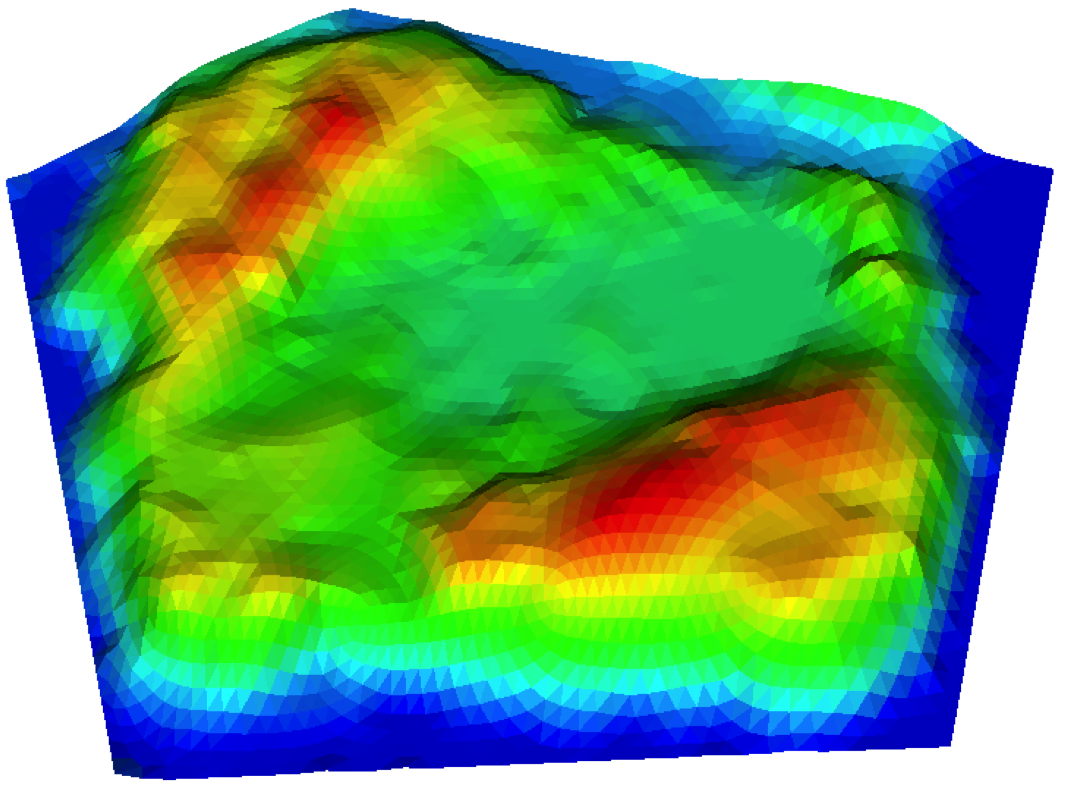
\includegraphics[width=11cm, height=6cm]{./figures/3DPolygonsImages/3Dpolygon40.png}
\caption{Microtopograpy for an example ice-wedge polygon from the Barrow Environmental Observatory (BEO).}
\label{3Dpolygon40}
\end{figure}

\begin{figure}
\centering
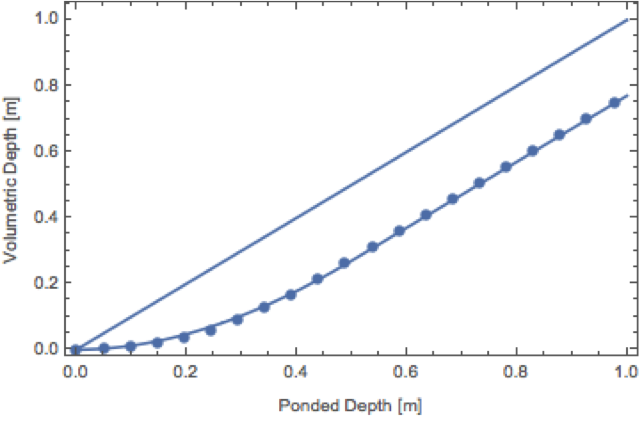
\includegraphics[width=12cm, height=8cm]{./figures/3DPolygonsImages/polygon40.png}
\caption{Volumetric depth versus ponded depth for polygon shown in Figure~\ref{3Dpolygon40}.}
\label{polygon40}
\end{figure}

\begin{figure}
\centering
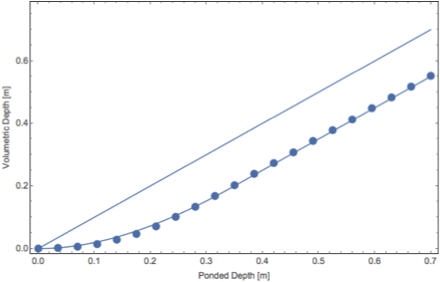
\includegraphics[width=6cm, height=6cm]{./figures/3DPolygonsImages/picture2.png}
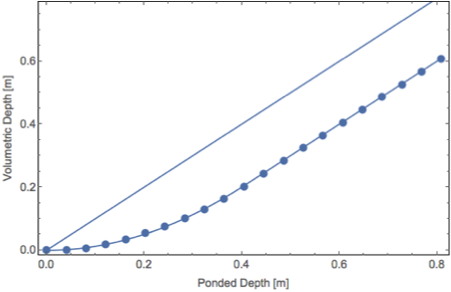
\includegraphics[width=6cm, height=6cm]{./figures/3DPolygonsImages/picture3.png}\\
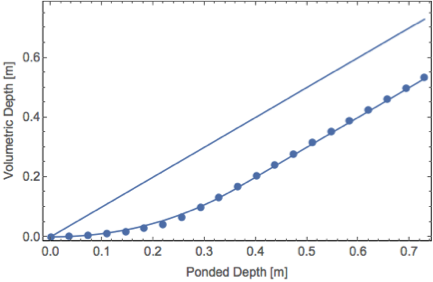
\includegraphics[width=6cm, height=6cm]{./figures/3DPolygonsImages/picture4.png}
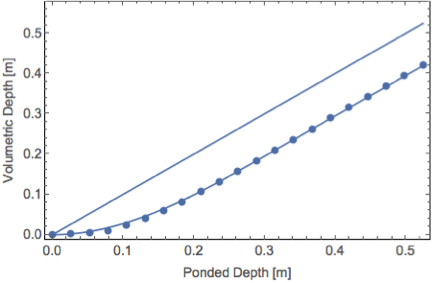
\includegraphics[width=6cm, height=6cm]{./figures/3DPolygonsImages/picture5.png}
\caption{Volumetric depth versus ponded depth for four additional ice-wedge polygons.}
\label{polygons}
\end{figure}

To calculate $\delta_\text{d}$ from the microtopography, we now propose an approach based on site percolation. Specifically, we fill the lowest elevation surface cells until the cluster of inundated cells spans the IWP. This is the percolation threshold. The water height at the percolation threshold defines the $\delta_\text{d}$. Figure~\ref{perc-cluster-poly40} shows the spanning cluster at the percolation threshold for the IWP of Figure~\ref{3Dpolygon40}. The depression depth calculated this way is 4.1 cm for this IWP.
It is reasonable to assume that the fractional conductance is well approximated by the fractional cross section available to flow, which can be estimated as the ratio of volumetric depth to ponded depth.

\begin{equation}
\Theta {(\delta_\text{d})} \approx \frac{( \Phi (\delta) - \Phi (\delta_\text{d}))} {\delta} H \left( \delta - \delta_\text{d}\right )
\end{equation}
Where $H$ is the Heaviside function. The numerator is the flowing cross sectional area. Note the velocity is multiplied by ponded depth to get a flux, so the molar flux appearing in the conservation equations becomes

\begin{equation}
\eta_{l} \delta U = - \eta_l  ( \Phi (\delta) - \Phi (\delta_\text{d})) H \left( \delta - \delta_\text{d}\right ) \Theta(\delta) \frac{(\delta - \delta_\text{d})^{2/3}}{n_\text{mann} (\| \nabla Z \| +\epsilon)^{1/2}} \nabla(Z + \delta)
\end{equation}
\begin{figure}
\centering
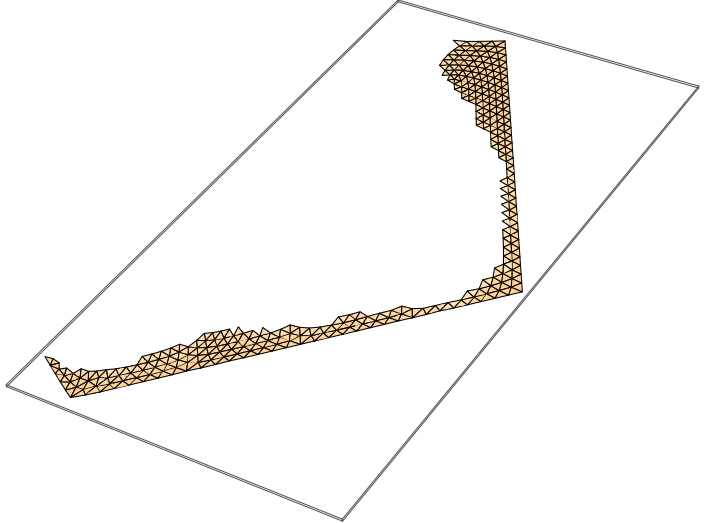
\includegraphics[width=12cm, height=6cm]{./figures/3DPolygonsImages/percolation-cluster-poly40.png}
\caption{The spanning cluster at the percolation threshold for the IWP of Figure~\ref{3Dpolygon40}. The water depth relative to the low point of the microtopography at the percolation threshold defines the depression depth.}
\label{perc-cluster-poly40}
\end{figure}

In summary, we hypothesize that the microtopographic effects on surface flow can be captured with a simple approximation with three parameters that can be computed from the microtopography:

\begin{itemize}
\item Subgrid relief $\delta_\text{max} = Z_{*,\text{max}} -   Z_{*,\text{min}}$, where  $Z_{*,\text{max}}$ and  $Z_{*,\text{min}}$ are the maximum and minimum elevation in the microtopography. 
\item Specific excluded volume $\delta_\text{ex}$, the soil volume above the microtopographic low point normalized by IWP area.
\item Depression depth $\delta$, the difference between the maximum and minimum elevation of the cells in the spanning cluster at the percolation threshold.
\end{itemize}
The subgrid releif and specific excluded volume come directly from the microtopography (univariate statistics). The depression depth requires a simple percolation algorithm to identify the spanning cluster at the percolation threshold. Values are given in Table~\ref{subgrid-para}.

\begin{center}
\begin{table}[htbp]
\caption{Parameters used in the subgrid model}\label{subgrid-para}
\begin{tabular}{| c |c|c|c|c|c|c|c|}
\hline
& C06 & C31 & C40 & C44 & C45 & A0 & B01 \\ \hline
 $\delta_\text{max}(m)$ & 0.404 & 0.262 & 0.483 & 0.364 & 0.350 & 0.361 & 0.411 \\ \hline
$\delta_\text{ex}(m)$ & 0.2 & 0.105 & 0.23 & 0.2 & 0.15 & 0.185 & 0.26\\ \hline
$ \delta_\text{d}(m)$ & 0.069 & 0.128 & 0.043 & 0.187 & 0.164 & 0.222 & 0.143 \\ \hline
\end{tabular}

\end{table}
\end{center}
\section{The Advanced Terrestrial Simulator (ATS)}\label{ATS}
\section{Numerical Results and Discussions}\label{numerical-tests}
\subsection{Simulations}
To assess the accuracy of the numerical results of our subgrid model, we compare our results with several fine-scale ice-wedge polygons and no subgrid results. To point out, the entire fine-scale IWP is considered as one grid cell in the subgrid and no subgrid model -- the slope depends on the elevation of the corners of the fine-scale IWP. For demonstration purpose, we consider surface-only flow simulations. In our work, the seven ice-wedge polygon for fine-scale simulations are considered from Barrow Environmental Observatory (BEO) and illustrated in Figures~~\ref{polygon40} and \ref{IWP-finescale}. These polygons consist of low-center, high-center, with well established troughs (relatively uniform elevation across the trough) and obstructions in the troughs, and hence represent a broader class of polygonal landscape. Three sets of numerical results of the subgrid model are presented:

\begin{description}\itemsep0pt \parskip0pt
\item [Study I:] Subgrid uncalibrated results;
\item [Study II:] Subgrid results with calibrated values of the depression depth listed in Table~\ref{subgrid-para};
\item [Study III:] Subgrid simulations with calibrated values of both the depression depth and the manning coefficient.
\end{description}

Study II is motivated by fine-scale simulations, higher depression depth may delay breakthrough, and would lead to more accumulation of water in the depressions, so it is important to reduce any uncertainty caused by the depression depth. On the other hand, higher pressure in the subgrid model affects the overland conductivity and more water is discharged in short time, to the mimic the behavior of the fine-scale after the breakthrough, the surface roughness is decreased by raising the manning coefficient in the governing equation; and motivates Study III.

Numerical simulations are performed for a  ``pulse numerical test" scenario -- injection followed by recession. In other words, we start with a fully dry surface, and inject water with a constant rate at the inlet boundary until breakthrough happens (prescribed flux boundary for a certain period of time), then stop the water supply and let water drain to the outlet (free drainage boundary). The arrows shown in Figure~\ref{IWP-finescale} indicate the inlet and outlet boundaries.

\subsection{Discussions}

Figure~\ref{polygon-C06} compares the numerical results of Study I and II with the fine-scale and no subgrid model. The results of the subgrid model yield a reasonable agreement with the fine-scale results as compared to the no subgrid model. The discharge curve of the fine-scale simulation has two peaks. When the inlet boundary has obstructions (for example, polygon C06 in Figure~\ref{IWP-finescale}) and divides the incoming water into different flow channels, the water reaches the outlet boundary at different times and lead to a dual-peak (or may be multiple peaks) hydrograph.  Due to only one grid cell in the subgrid model, the dual-peak behavior is not possible to capture. The high overland conductivity in the subgrid model is reduced by increasing the surface roughness (i.e., the manning coefficient). It improves the results and replicate the recession period of the fine-scale results. It is important to see the amount of water (not available for drainage) in the system after the recession period. Figure~\ref{polygon-C06} also displays the water retained the in subgrid model and the fine-scale model -- the match is very close. It is important to point out that the recession period consistently needs the surface roughness to be adjusted in all the results reported here. \\
Numerical simulations correspond to polygon C31 are shown in Figure~\ref{polygon-C31}. For polygon C31, the results of the subgrid model are strongly affected by the depression depth in Study I, and lead to a mismatch. However, the results of Study II and III indicate that calibrated values of the depression depth and the surface roughness improved the simulated results dramatically and yield a close match. \\ %discuss why the percolation algorithm provided a high depression depth.
Numerical results of polygons (C40, C44, C45, A01, and B01) are shown in Figures~\ref{polygon-C40}, \ref{polygon-C44}, \ref{polygon-C45}, \ref{polygon-A01}, and \ref{polygon-B01}, respectively. displays the numerical results of Study I and II of polygon C40. Overall, the calibrated results (Study III) consistently show a better fit to the fine-scale simulations.

%\subsection{Summary}
\itemize{

\item Increased surface roughness in the subgrid model positively affects the results -- an indication of a needed drag coefficient in the flow law. A relatively smooth discharge curve is a consequence of a lower gradient between the cell center and outlet boundary.

\item For low-centered polygons such as C45 adn A01, Study I (uncalibrated results) fails to match the hydrograph of the fine-scale simulations -- no breakthrough happens for the uncalibrated depression depths. Fine-scale simulations show that low-elevated regions may remain completely dry if they are not located in the main flow channel. However, our percolation algorithm computes the depression depth provided low-elevated spots are filled with water and a cluster is formed. In such scenario, the uncalibrated depression depths  need to be decreased by a factor of 2-3

\item Application of invaded percolation (flow in the direction of least resistance) algorithm could provide more accurate depression depths such that the subgrid simulated results replicate the fine-scale results without any calibration.

\item A low-centered polygon with lowest elevation in the center and obstructions in the troughs are lowered than the raised rims, see for example polygon A01, the computed depression depth requires to be decreased by a factor of 3.
} 

%As said earlier, as long as the ice-wedge trough is well established the percolation algorithm provides reasonably accurate values of the depression depth and hence the breakthrough in the fine-scale and the subgrid model happens around the same time.  Also, the increased surface roughness positively affects the discharge curve at the breakthrough time. A


%it is a high-centered polygon As we see experiments yielded equally good results for one-step and multistep desorption. Moreover, the addition of soil water pressure head data resulted in unique par

%POLYG31: Elevation: Min=4.510, Max = 4.772
%POLY_A: Elevation: Min = 5.134, Max = 5.495
%POLY_B: Elevation: Min = 5.025, Max = 5.436
\begin{figure}
\centering
\vskip -1cm
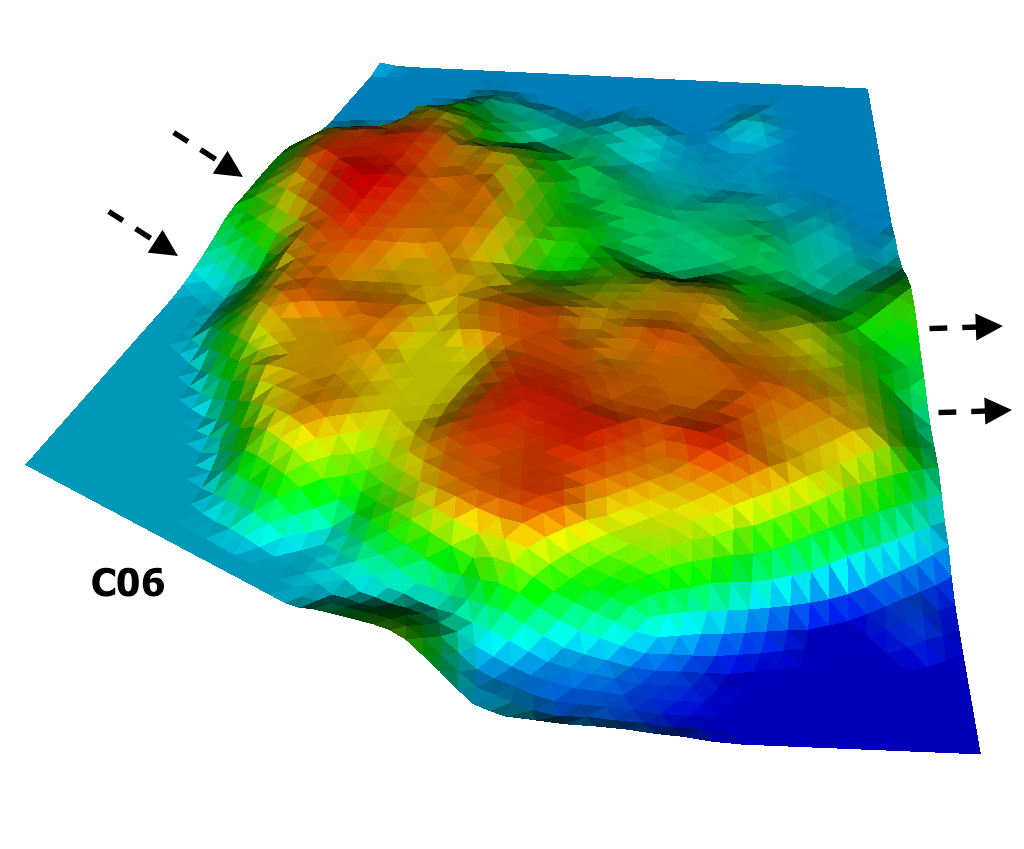
\includegraphics[width=6.2cm, height=6cm]{./figures/3DPolygonsImages/3Dpolygon06-3B.png}
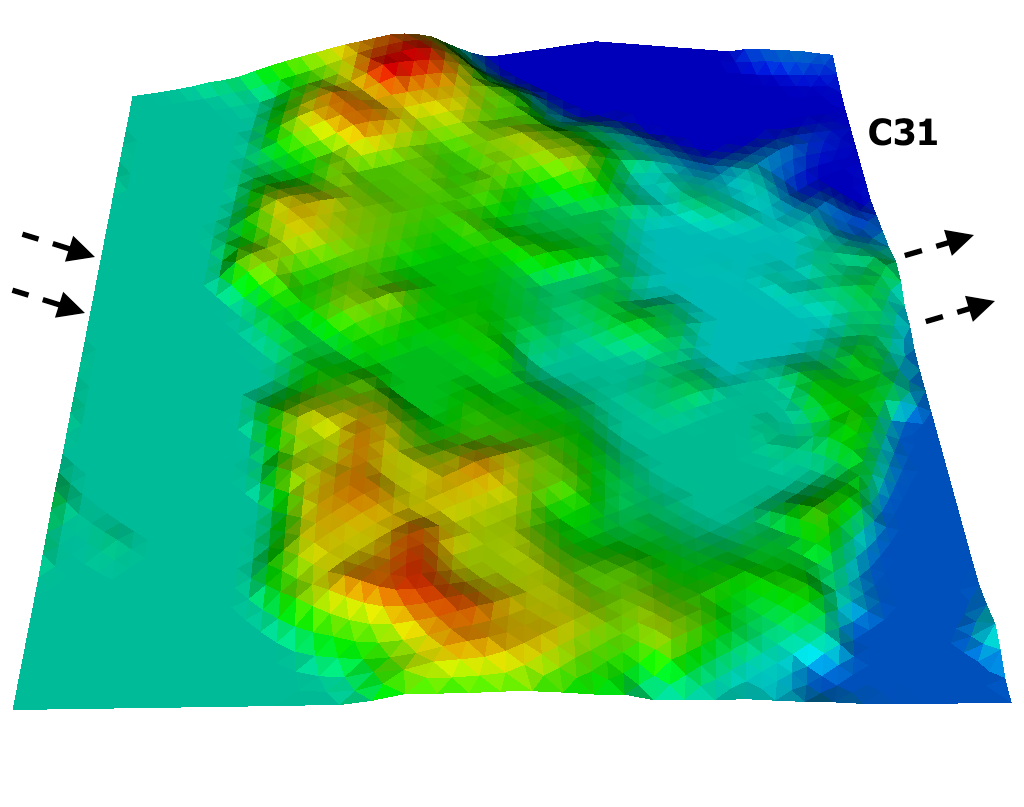
\includegraphics[width=6.2cm, height=6cm]{./figures/3DPolygonsImages/3Dpolygon31-3B.png}\\
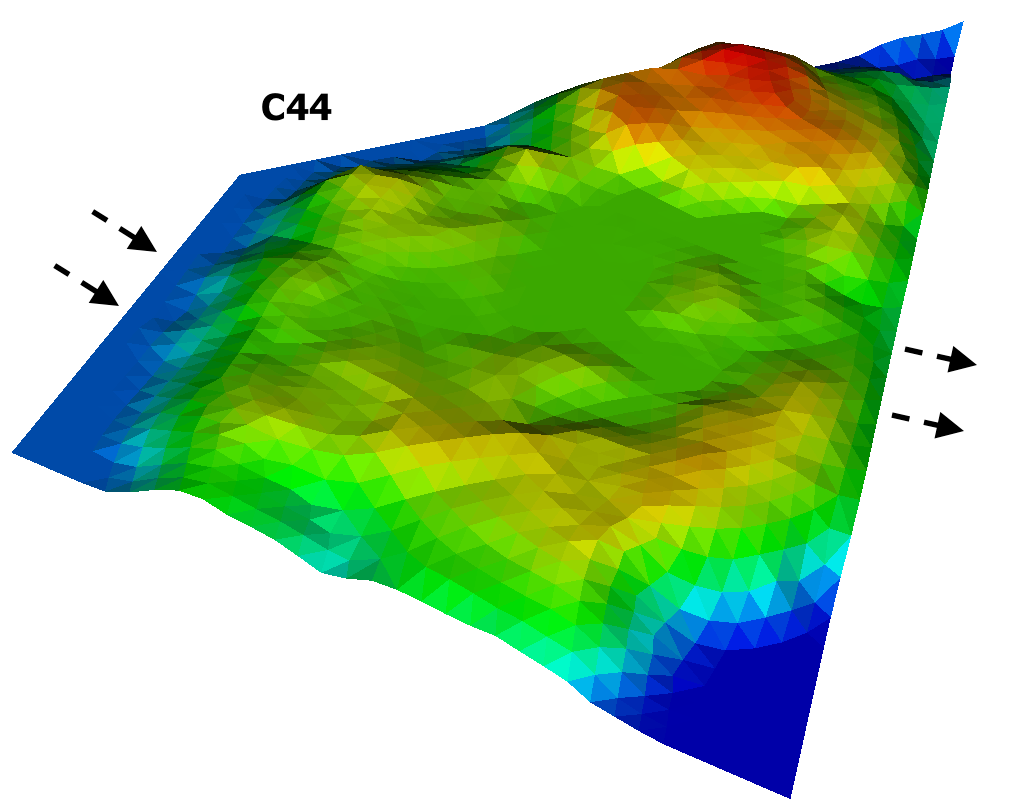
\includegraphics[width=6.cm, height=6cm]{./figures/3DPolygonsImages/3Dpolygon44-3B.png}
\hskip -0.4cm 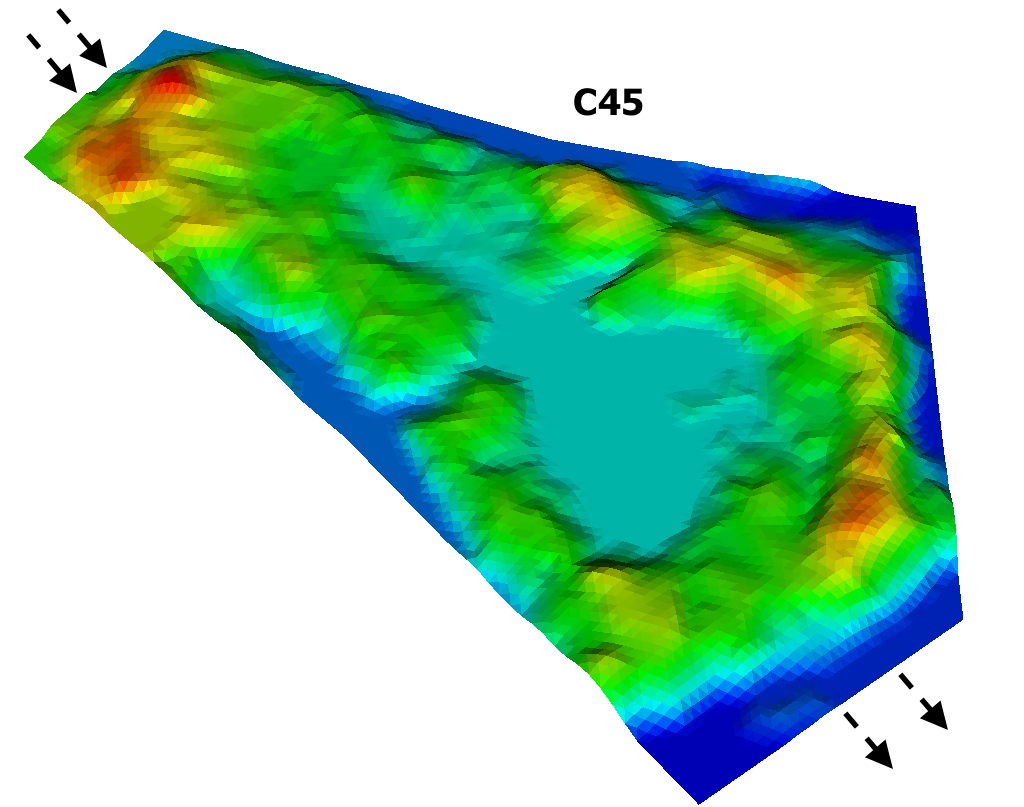
\includegraphics[width=6.8cm, height=6cm]{./figures/3DPolygonsImages/3Dpolygon45-3B.png}\\
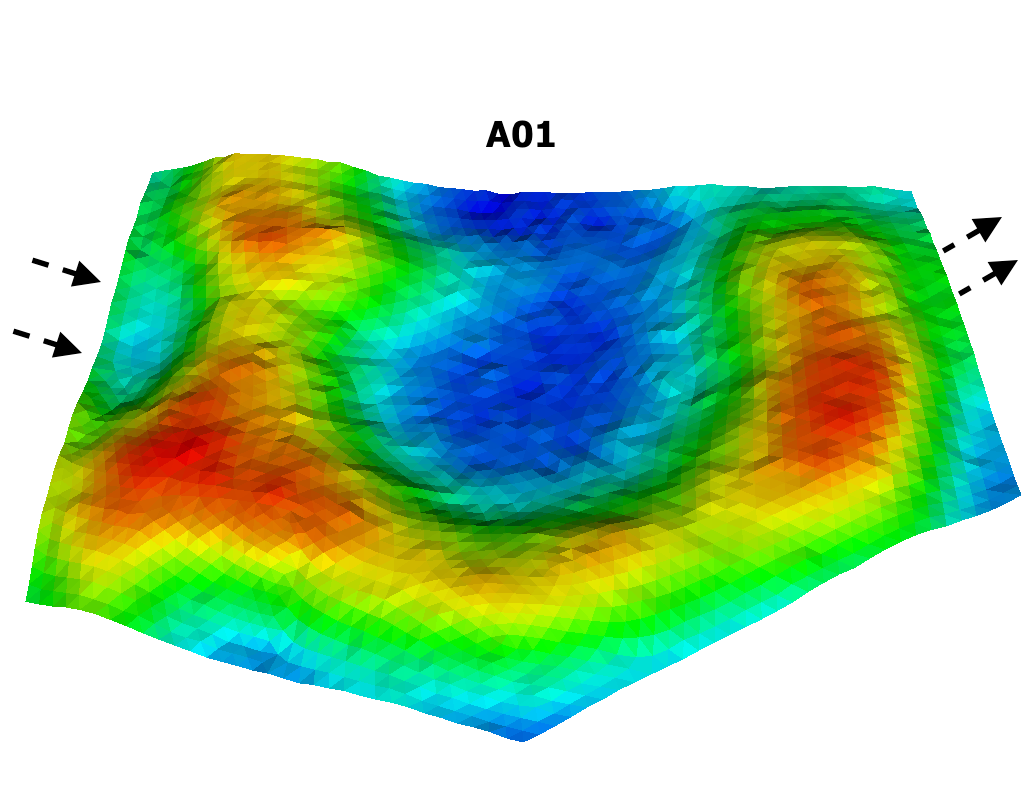
\includegraphics[width=6.2cm, height=6cm]{./figures/3DPolygonsImages/3DpolygonA01-3B.png}
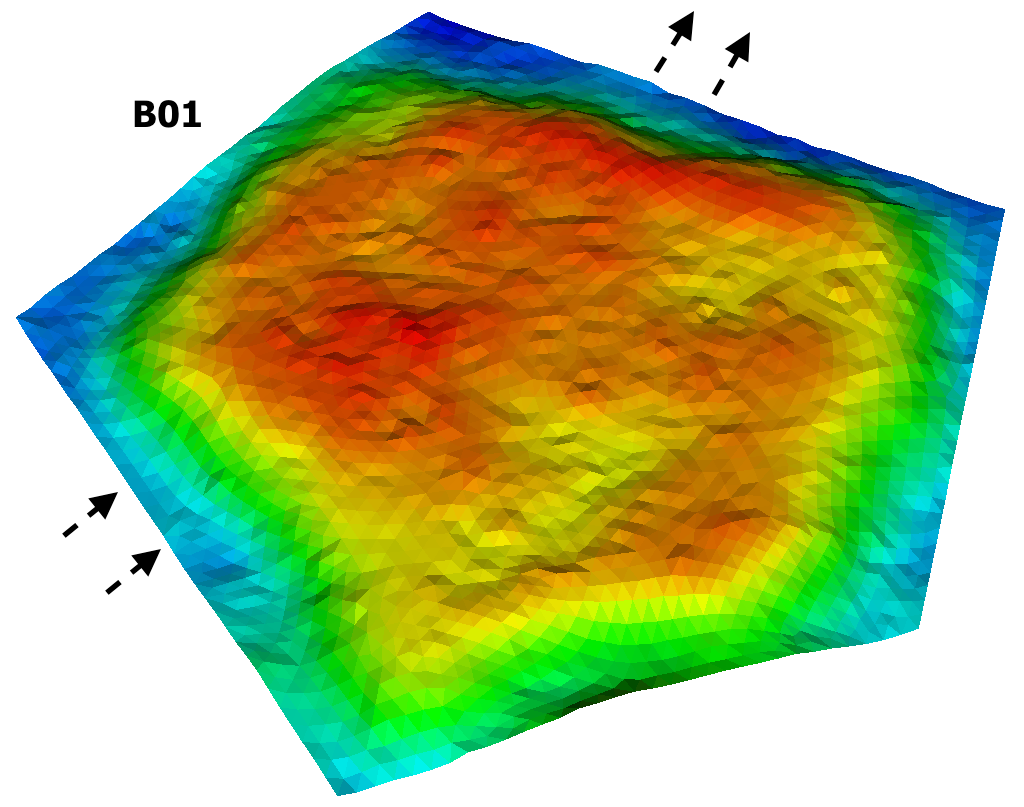
\includegraphics[width=6.2cm, height=6cm]{./figures/3DPolygonsImages/3DpolygonB01-3B.png}
\caption{An Illustration of the microtopography for ice-wedge polygons from Barrow Environmental Observatory (BEO). Red and dark blue spots correspond to high- and low-elevated regions. The arrows indicate inlet and outlet boundaries.}
\label{IWP-finescale}
\end{figure}

%These results do not clearly indicate
\begin{figure}
\centering
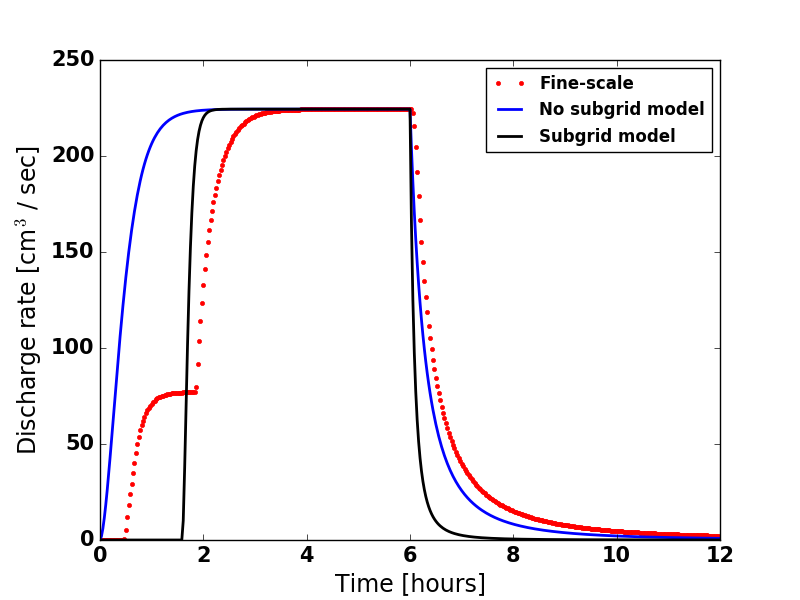
\includegraphics[width=6.2cm, height=6cm]{./figures/POLYGON06/POLYGON06discharge.png}
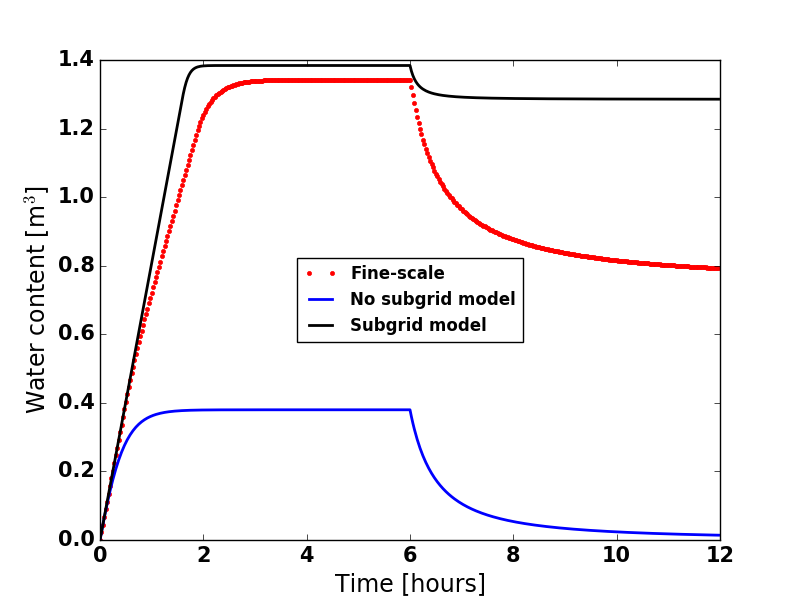
\includegraphics[width=6.2cm, height=6cm]{./figures/POLYGON06/POLYGON06watercontent.png}\\
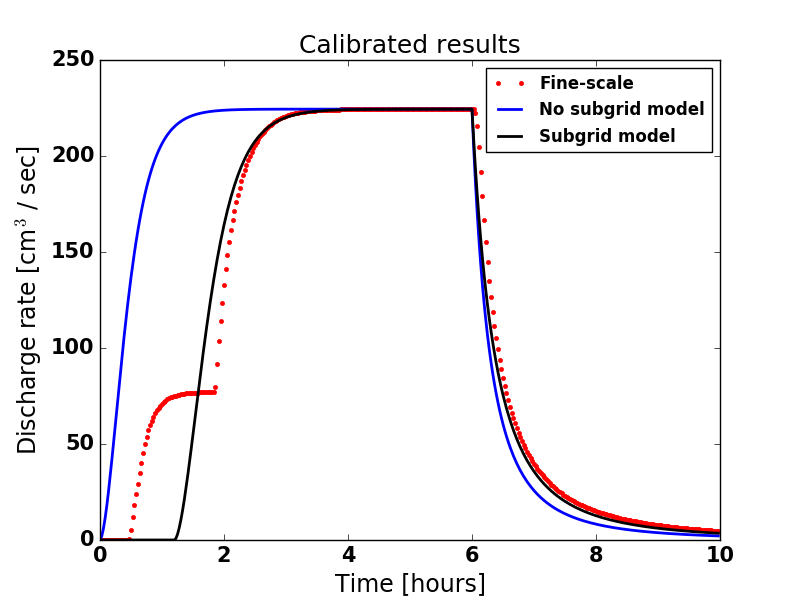
\includegraphics[width=6.2cm, height=6cm]{./figures/POLYGON06/POLYGON06dischargeCalibDDManning.png}
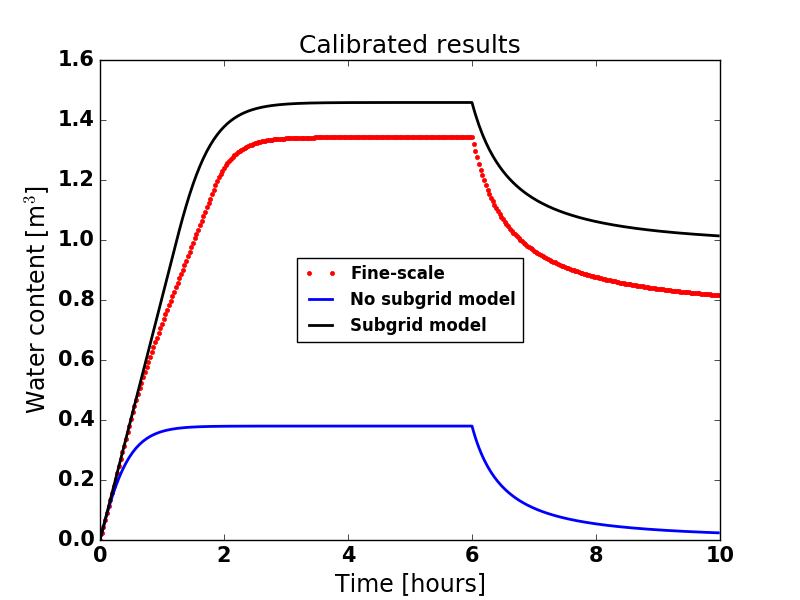
\includegraphics[width=6.2cm, height=6cm]{./figures/POLYGON06/POLYGON06watercontentCalibDDManning.png}
\caption{(Polygon C06) Comparison of the numerical results of the subgrid model with the fine-scale and without subgrid model results. Bottom row displays calibrated results of Study II.}
\label{polygon-C06}
\end{figure}


\begin{figure}
\centering
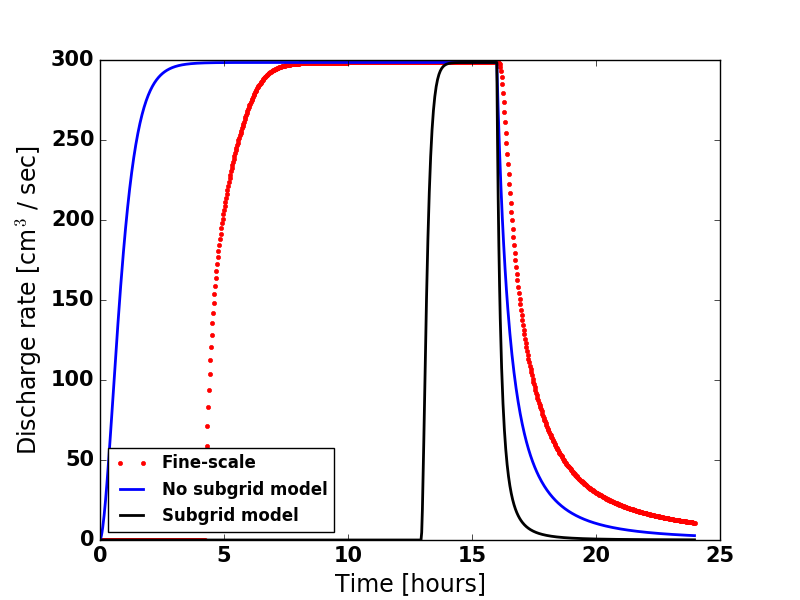
\includegraphics[width=6.2cm, height=5cm]{./figures/POLYGON31/POLYGON31discharge.png}
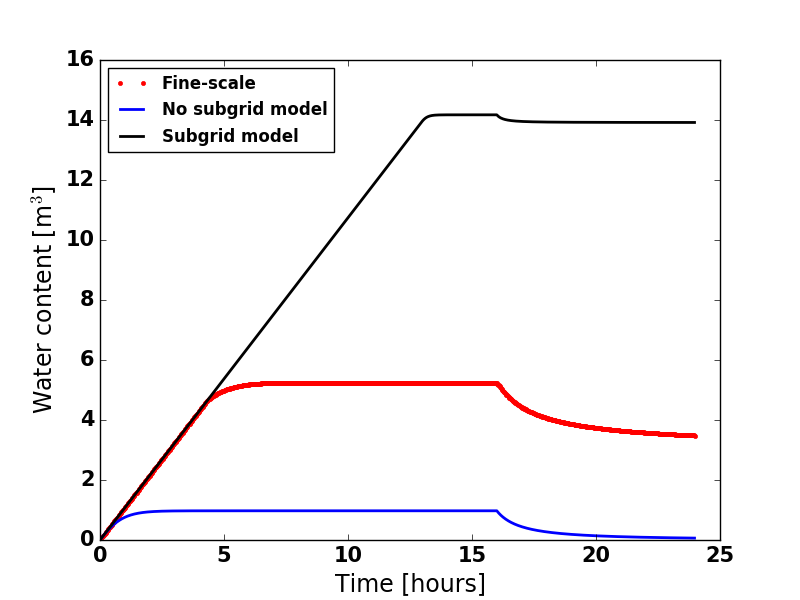
\includegraphics[width=6.2cm, height=5cm]{./figures/POLYGON31/POLYGON31watercontent.png}\\
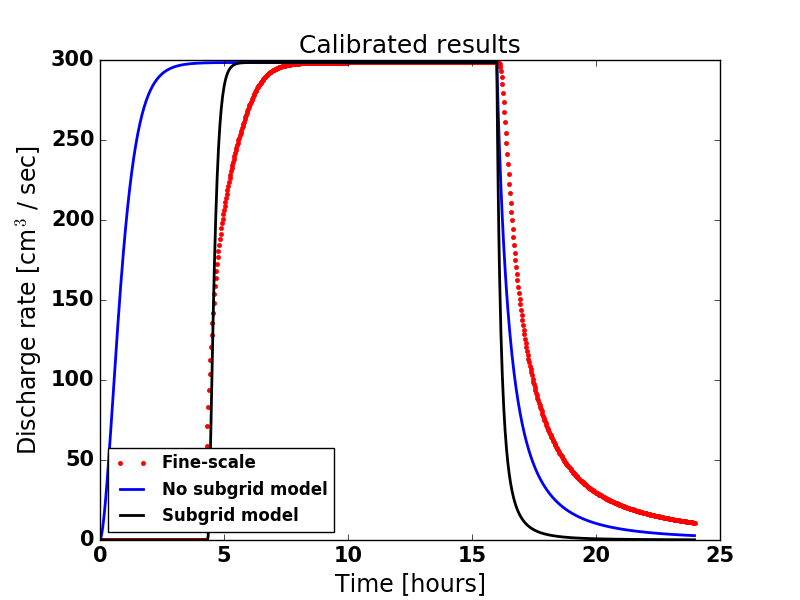
\includegraphics[width=6.2cm, height=5cm]{./figures/POLYGON31/POLYGON31dischargeCalibDD.png}
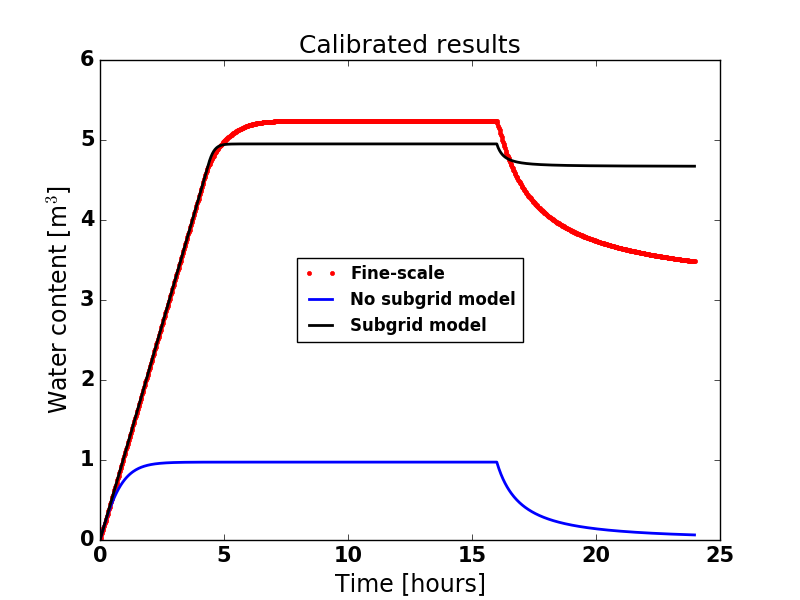
\includegraphics[width=6.2cm, height=5cm]{./figures/POLYGON31/POLYGON31watercontentCalibDD.png} \\
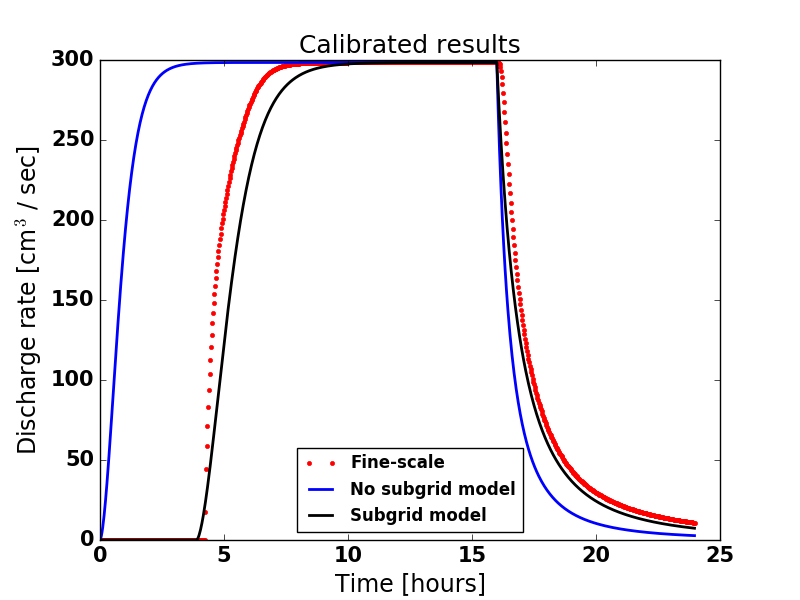
\includegraphics[width=6.2cm, height=5cm]{./figures/POLYGON31/POLYGON31dischargeCalibDDManning.png}
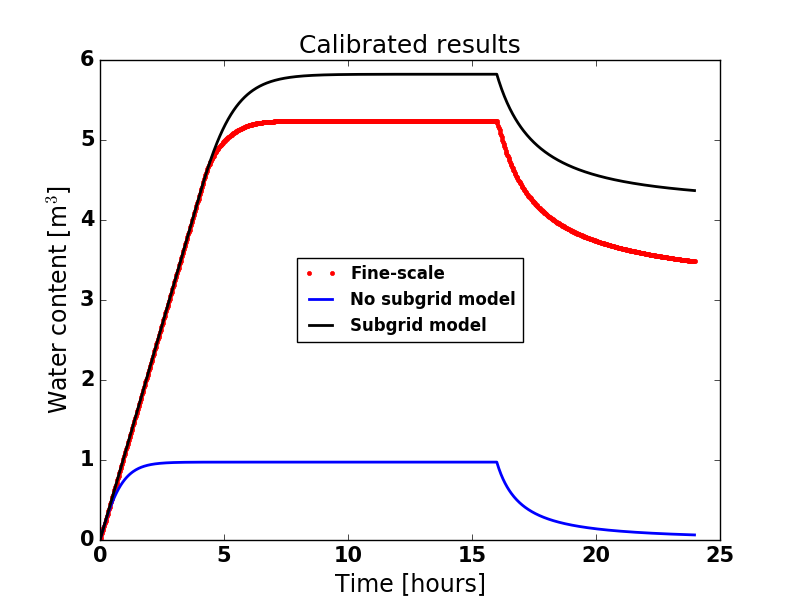
\includegraphics[width=6.2cm, height=5cm]{./figures/POLYGON31/POLYGON31watercontentCalibDDManning.png}
\caption{(Polygon C31) Comparison of the numerical results of the subgrid model with the fine-scale and without subgrid model results. Middle row (Study II): Calibrated value of the depression depth. Bottom row (Study III): Calibrated value of the depression depth and the manning coefficient.}
\label{polygon-C31}
\end{figure}


\begin{figure}
\centering
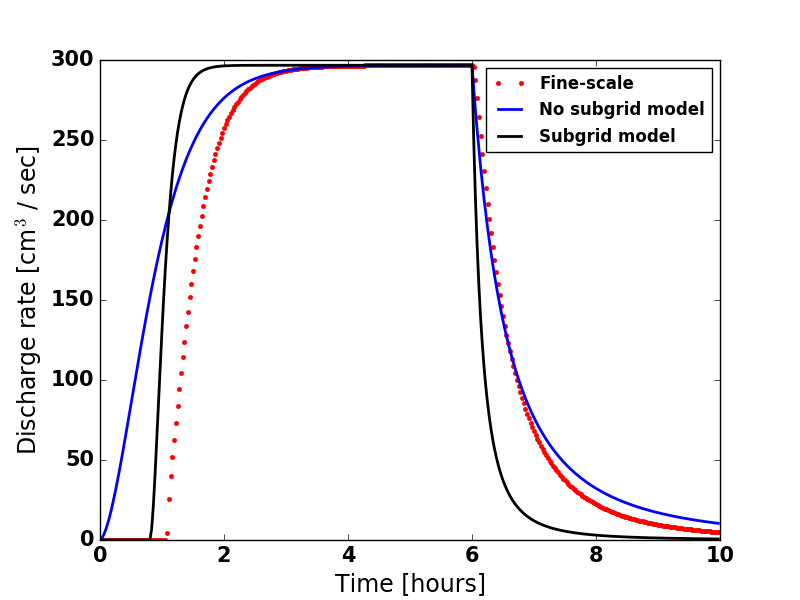
\includegraphics[width=6.2cm, height=5.5cm]{./figures/POLYGON40/POLYGON40discharge.png}
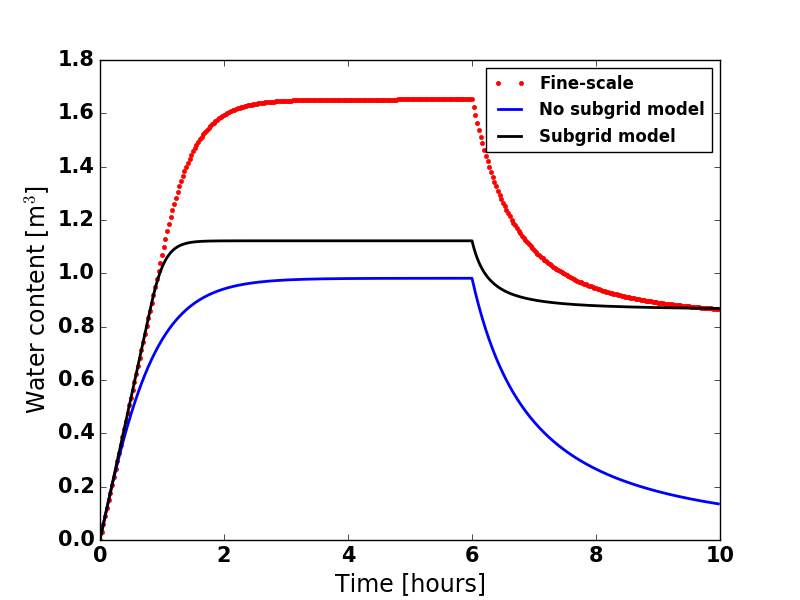
\includegraphics[width=6.2cm, height=5.5cm]{./figures/POLYGON40/POLYGON40watercontent.png}\\
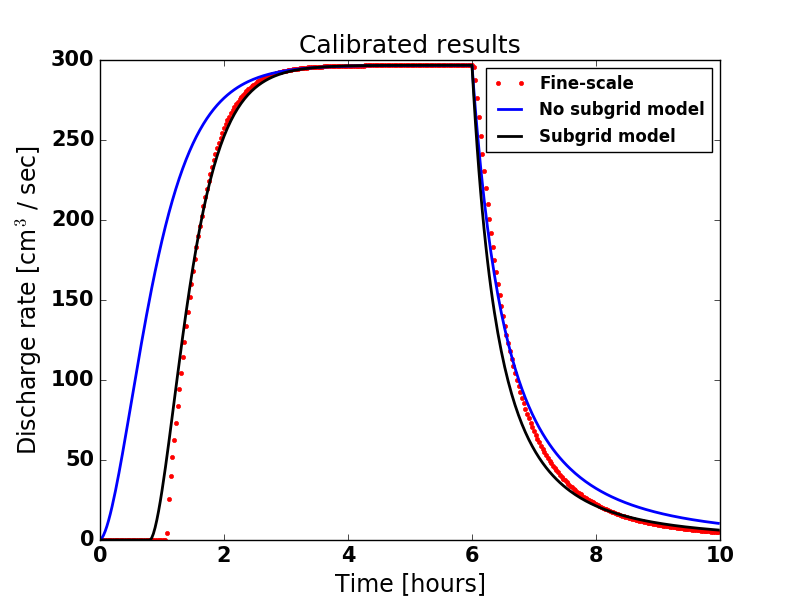
\includegraphics[width=6.2cm, height=5.5cm]{./figures/POLYGON40/POLYGON40dischargeCalibManning.png}
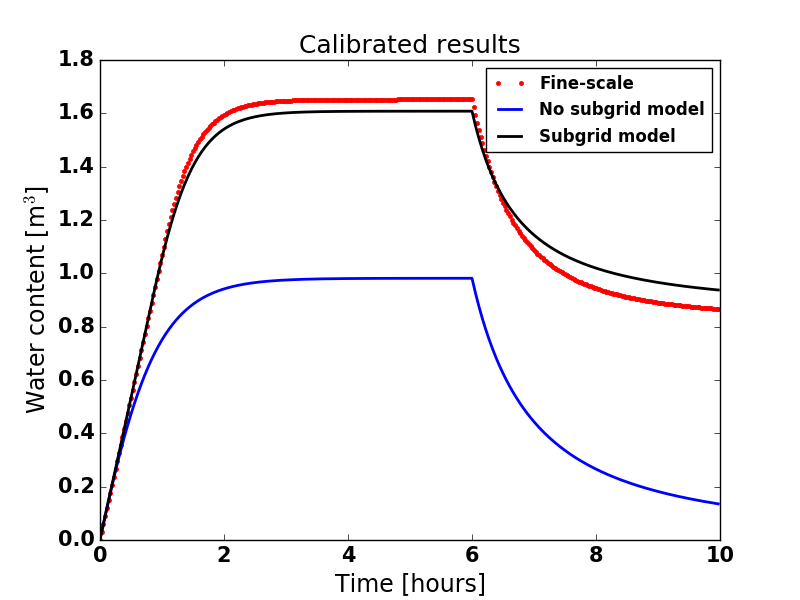
\includegraphics[width=6.2cm, height=5.5cm]{./figures/POLYGON40/POLYGON40watercontentCalibManning.png}
\caption{(Polygon C40) Comparison of the numerical results of the subgrid model with the fine-scale and without subgrid model results. Bottom row displays calibrated results.}
\label{polygon-C40}
\end{figure}

\begin{figure}
\centering
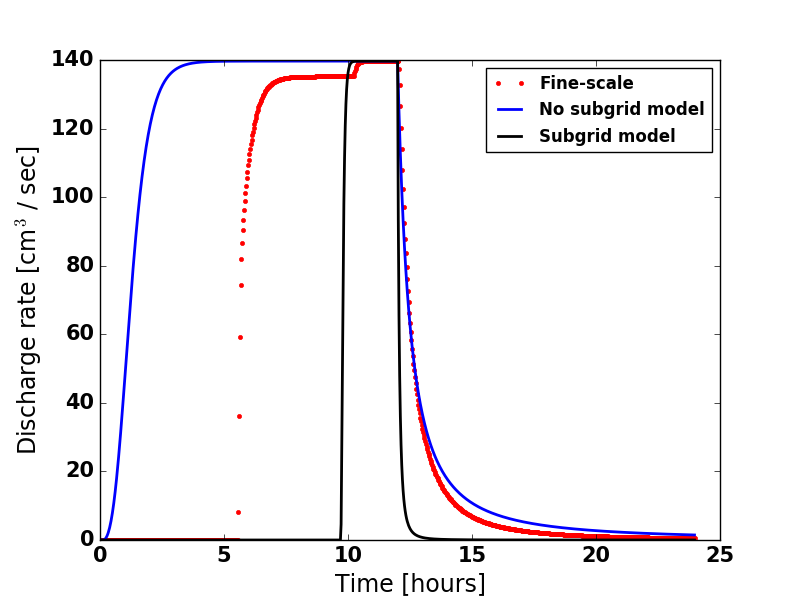
\includegraphics[width=6.2cm, height=5.5cm]{./figures/POLYGON44/POLYGON44discharge.png}
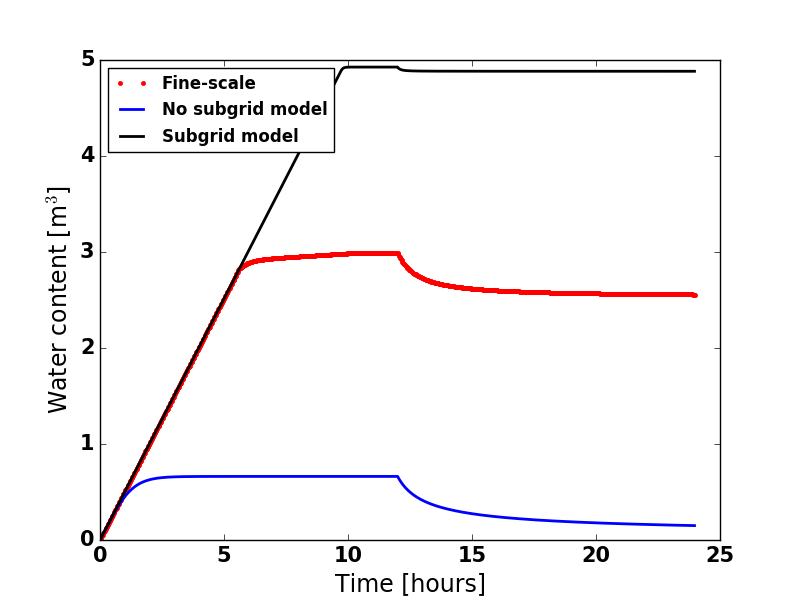
\includegraphics[width=6.2cm, height=5.5cm]{./figures/POLYGON44/POLYGON44watercontent.png}\\
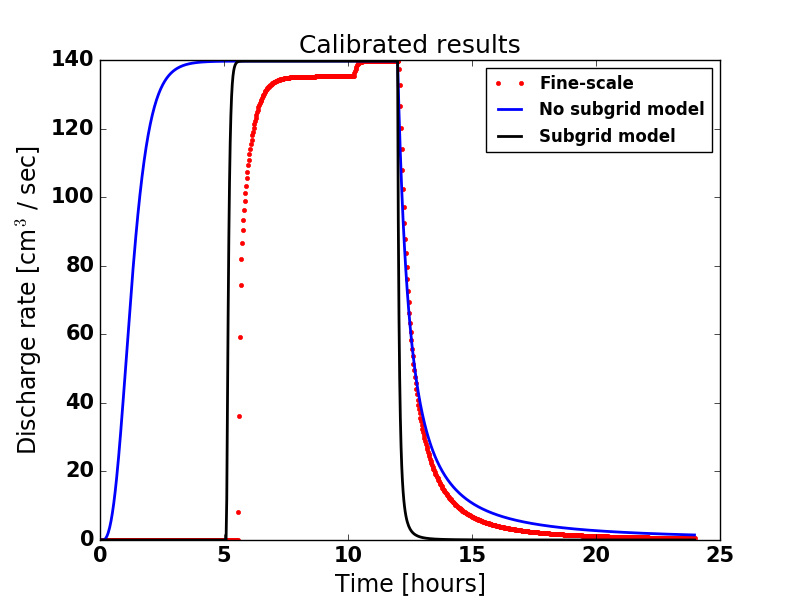
\includegraphics[width=6.2cm, height=5.5cm]{./figures/POLYGON44/POLYGON44dischargeCalibDD.png}
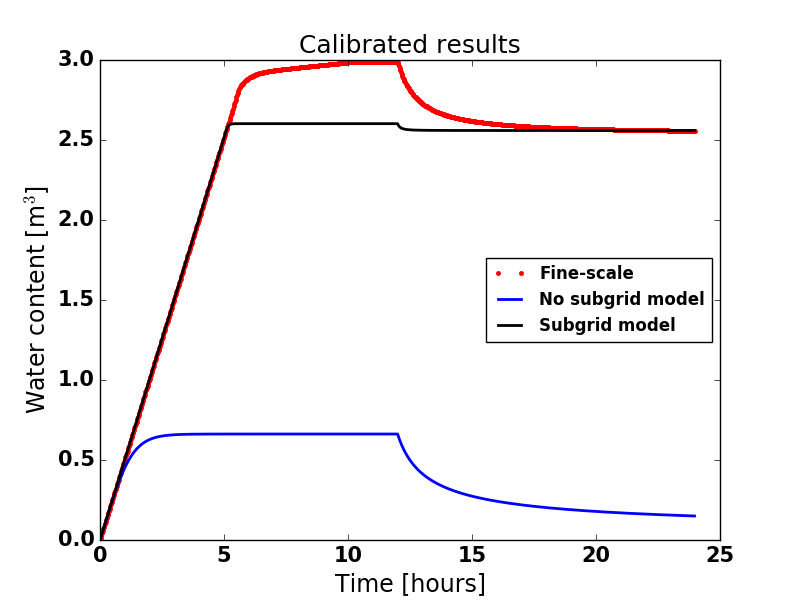
\includegraphics[width=6.2cm, height=5.5cm]{./figures/POLYGON44/POLYGON44watercontentCalibDD.png} \\
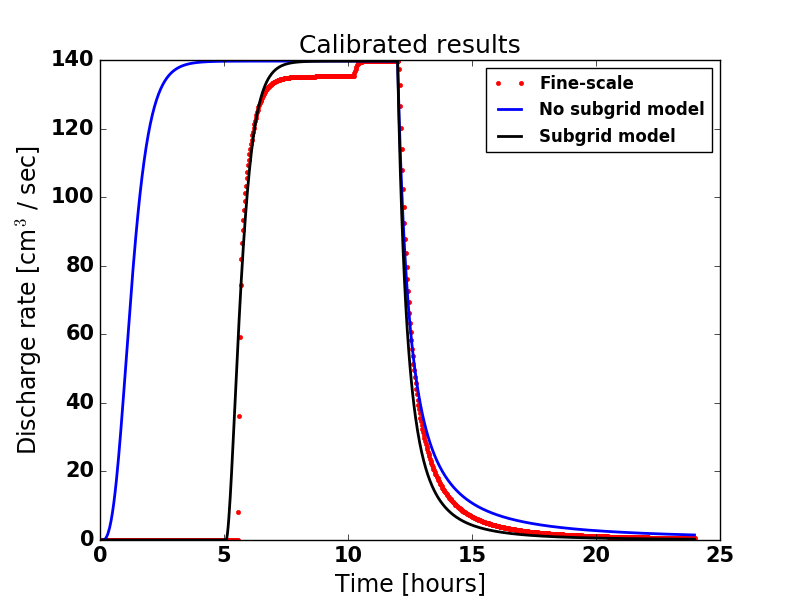
\includegraphics[width=6.2cm, height=5.5cm]{./figures/POLYGON44/POLYGON44dischargeCalibDDManning.png}
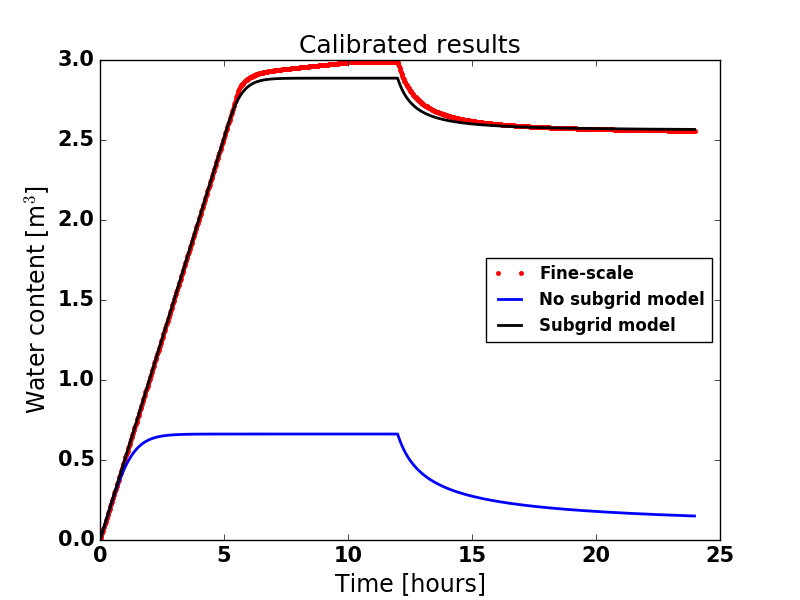
\includegraphics[width=6.2cm, height=5.5cm]{./figures/POLYGON44/POLYGON44watercontentCalibDDManning.png}
\caption{(Polygon C44) Comparison of the numerical results of the subgrid model with the fine-scale and without subgrid model results. Middle row: Calibrated value of the depression depth. Bottom row: Calibrated value of the depression depth and the manning coefficient.}
\label{polygon-C44}
\end{figure}


\begin{figure}[!h]
\centering
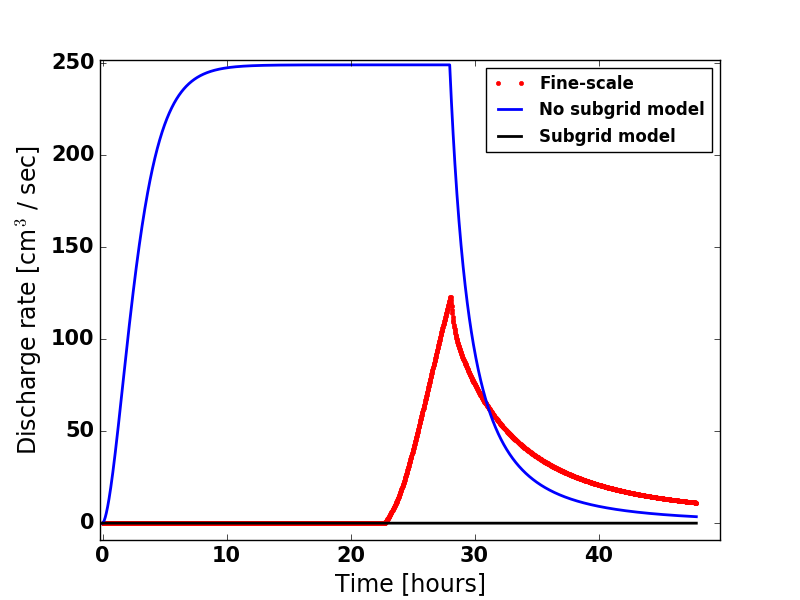
\includegraphics[width=6.2cm, height=5.5cm]{./figures/POLYGON45/POLYGON45discharge2.png}
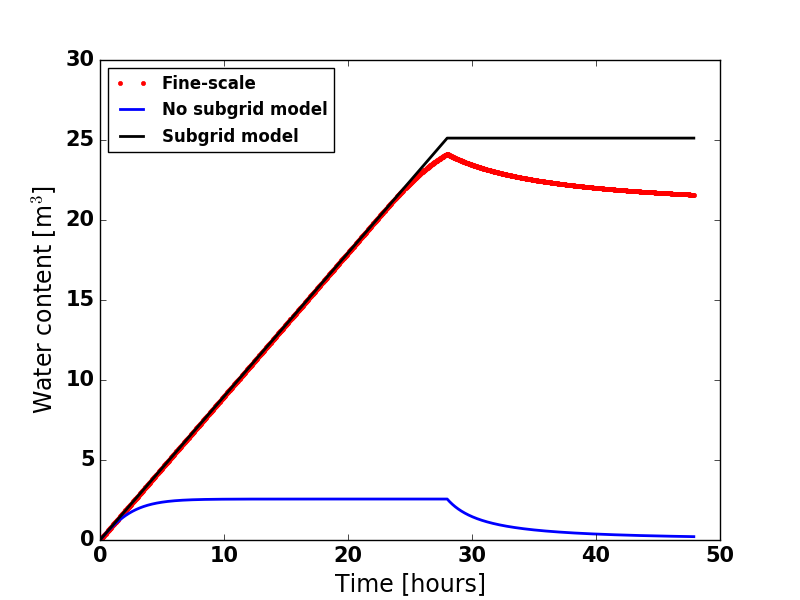
\includegraphics[width=6.2cm, height=5.5cm]{./figures/POLYGON45/POLYGON45watercontent.png}\\
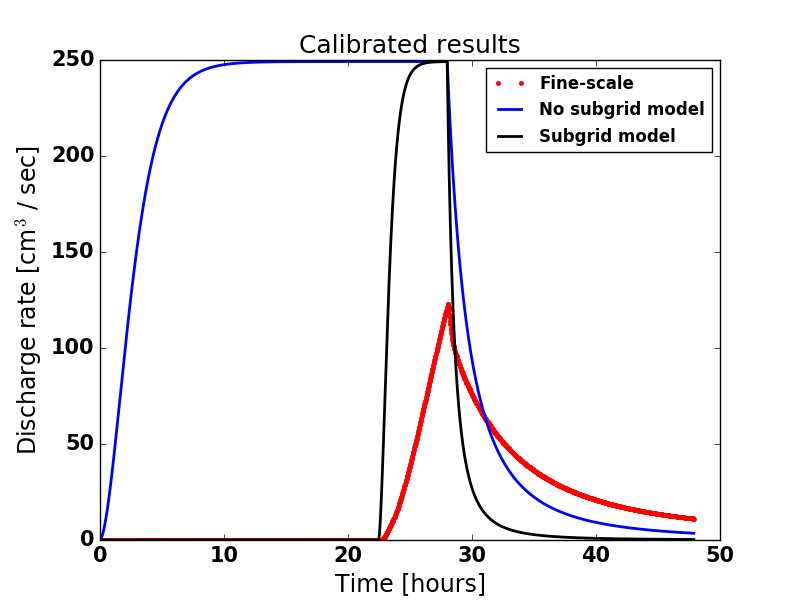
\includegraphics[width=6.2cm, height=5.5cm]{./figures/POLYGON45/POLYGON45dischargeCalibDD.png}
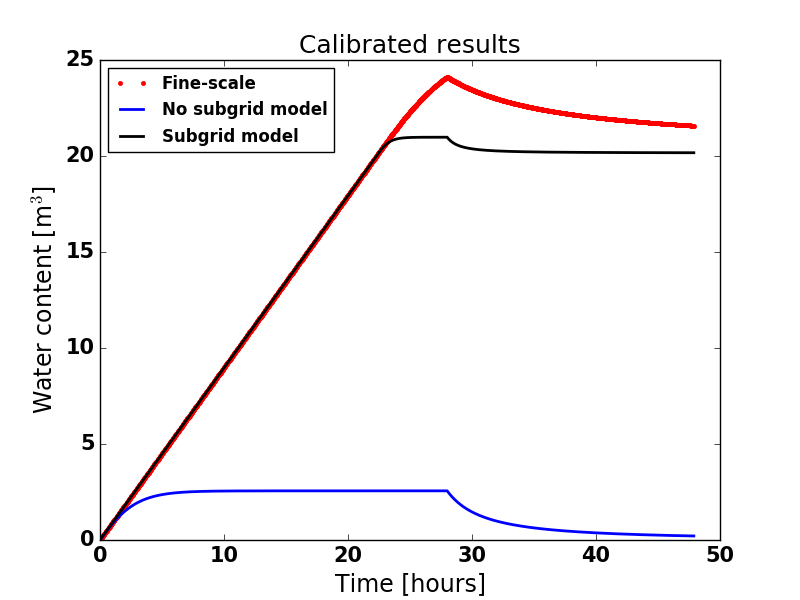
\includegraphics[width=6.2cm, height=5.5cm]{./figures/POLYGON45/POLYGON45watercontentCalibDD.png} \\
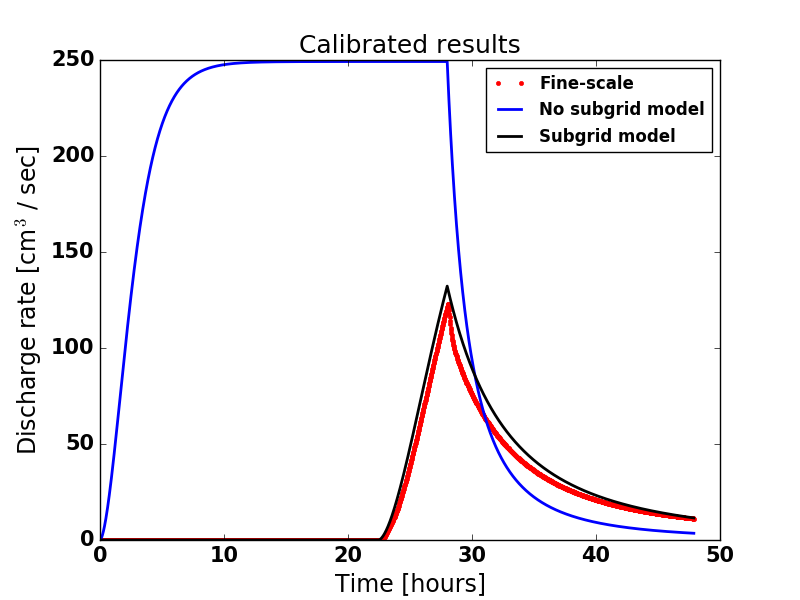
\includegraphics[width=6.2cm, height=5.5cm]{./figures/POLYGON45/POLYGON45dischargeCalibDDManning.png}
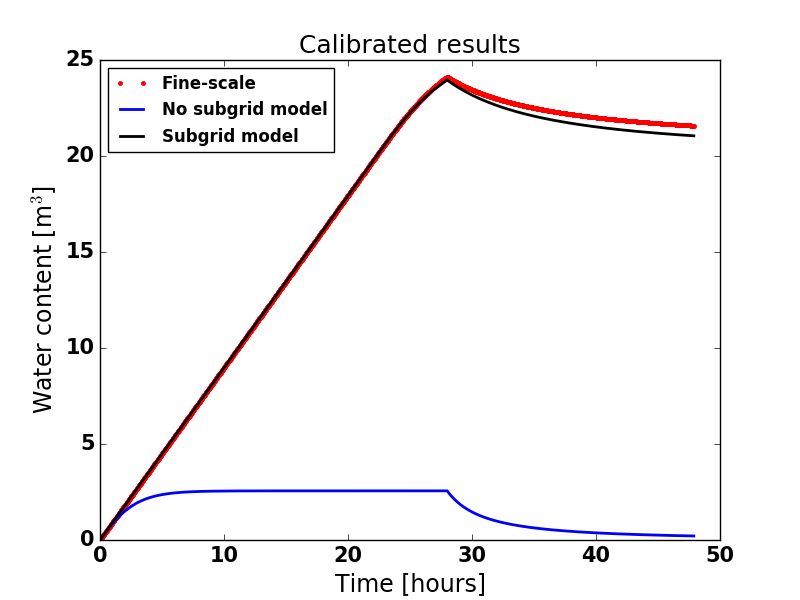
\includegraphics[width=6.2cm, height=5.5cm]{./figures/POLYGON45/POLYGON45watercontentCalibDDManning.png}
\caption{(Polygon C45) Comparison of the numerical results of the subgrid model with the fine-scale and without subgrid model results. Middle row: Calibrated value of the depression depth. Bottom row: Calibrated value of the depression depth and the manning coefficient.}
\label{polygon-C45}
\end{figure}




\begin{figure}[!h]
\centering
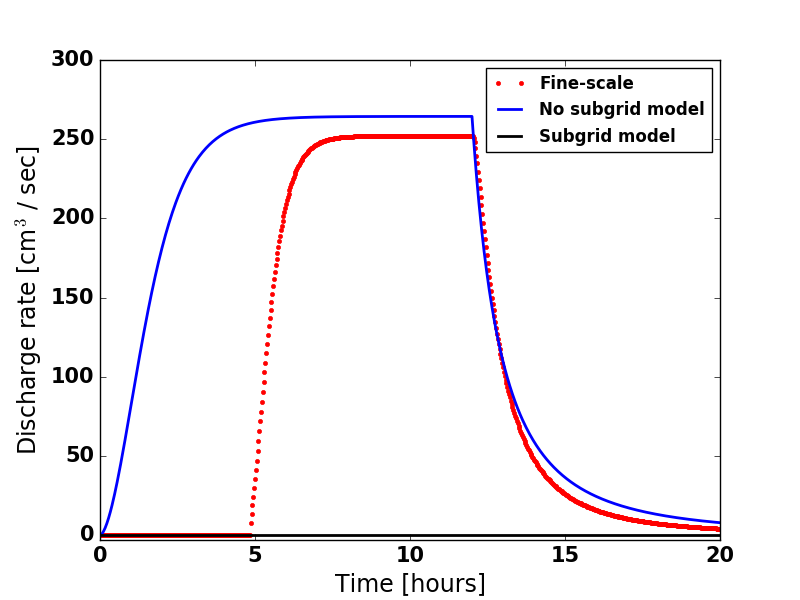
\includegraphics[width=6.2cm, height=5.5cm]{./figures/POLYGON_A01/POLYGON_A01discharge.png}
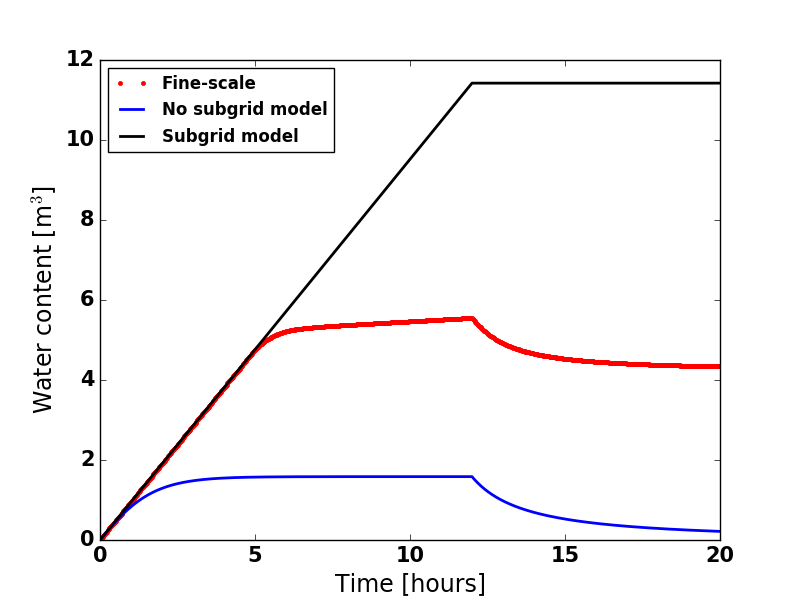
\includegraphics[width=6.2cm, height=5.5cm]{./figures/POLYGON_A01/POLYGON_A01watercontent.png}\\
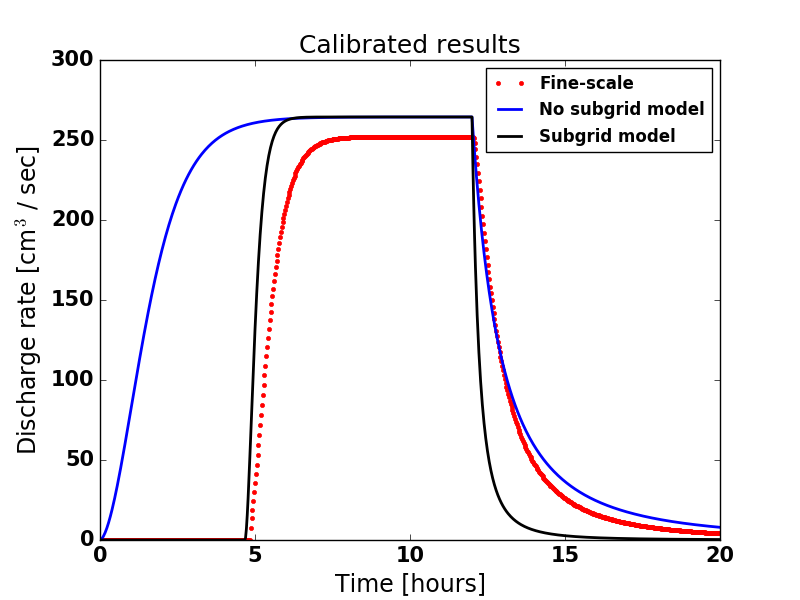
\includegraphics[width=6.2cm, height=5.5cm]{./figures/POLYGON_A01/POLYGON_A01dischargeCalibDD.png}
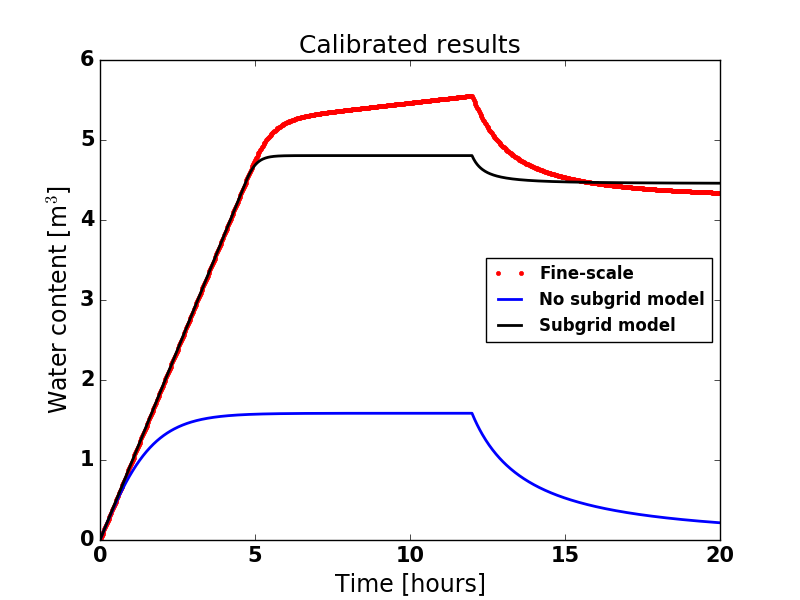
\includegraphics[width=6.2cm, height=5.5cm]{./figures/POLYGON_A01/POLYGON_A01watercontentCalibDD.png} \\
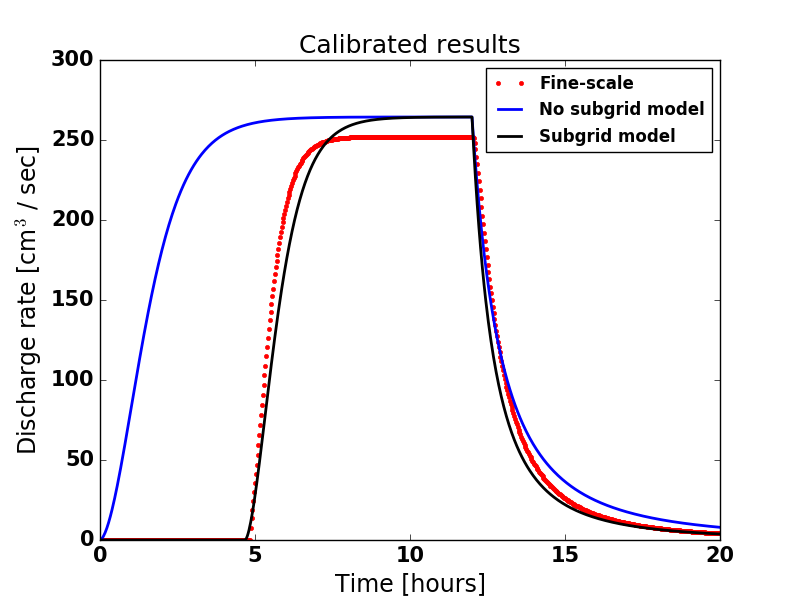
\includegraphics[width=6.2cm, height=5.5cm]{./figures/POLYGON_A01/POLYGON_A01dischargeCalibDDManning.png}
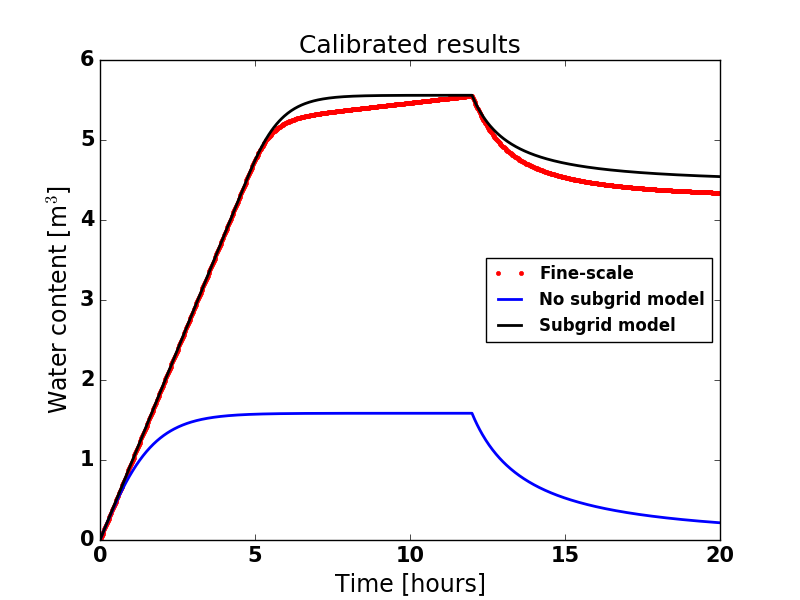
\includegraphics[width=6.2cm, height=5.5cm]{./figures/POLYGON_A01/POLYGON_A01watercontentCalibDDManning.png}
\caption{(Polygon A01) Comparison of the numerical results of the subgrid model with the fine-scale and without subgrid model results. Middle row: Calibrated value of the depression depth. Bottom row: Calibrated value of the depression depth and the manning coefficient.}
\label{polygon-A01}
\end{figure}



\begin{figure}[!h]
\centering
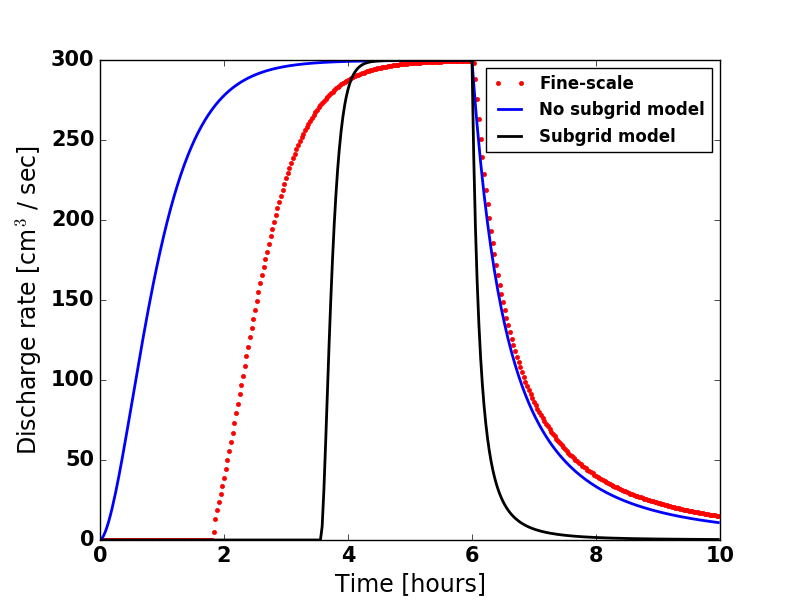
\includegraphics[width=6.2cm, height=5.5cm]{./figures/POLYGON_B01/POLYGON_B01discharge.png}
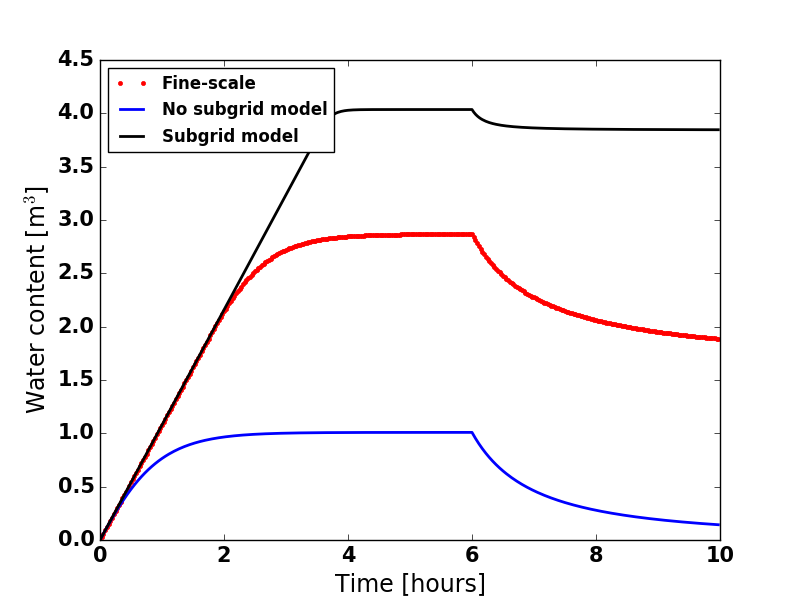
\includegraphics[width=6.2cm, height=5.5cm]{./figures/POLYGON_B01/POLYGON_B01watercontent.png}\\
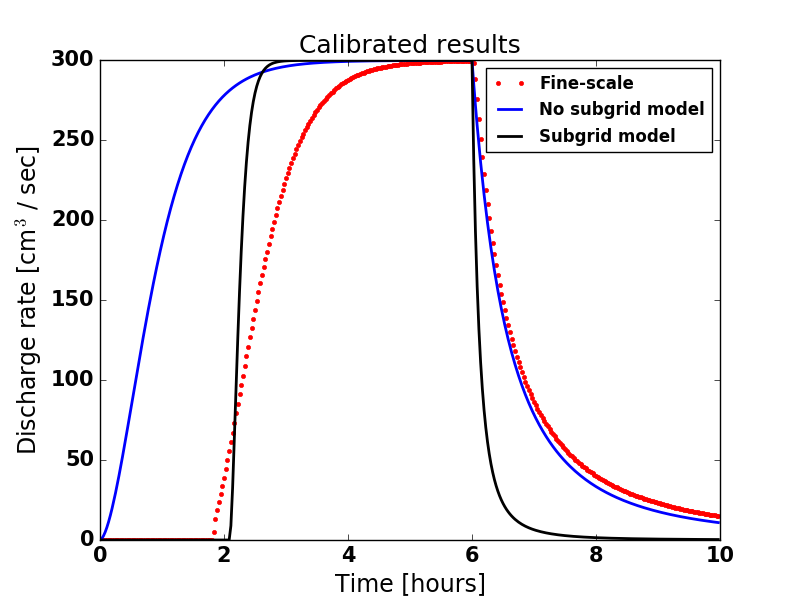
\includegraphics[width=6.2cm, height=5.5cm]{./figures/POLYGON_B01/POLYGON_B01dischargeCalibDD.png}
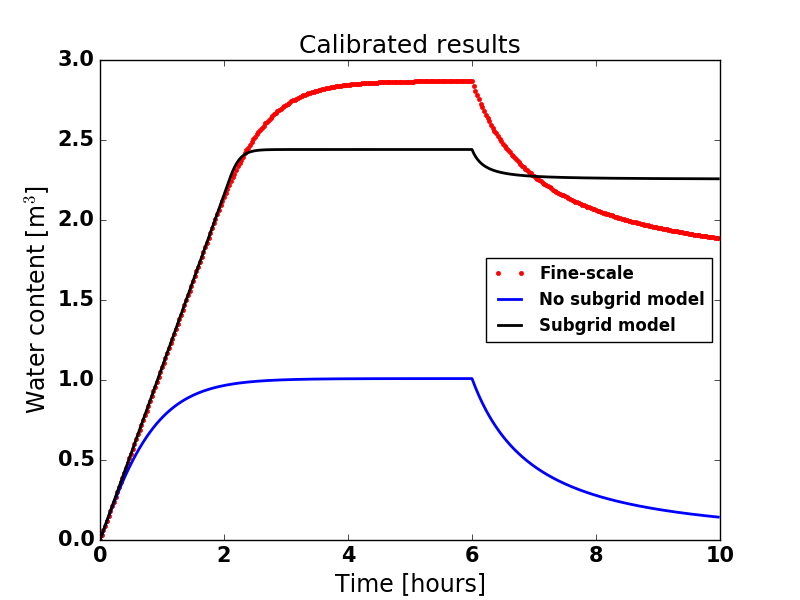
\includegraphics[width=6.2cm, height=5.5cm]{./figures/POLYGON_B01/POLYGON_B01watercontentCalibDD.png} \\
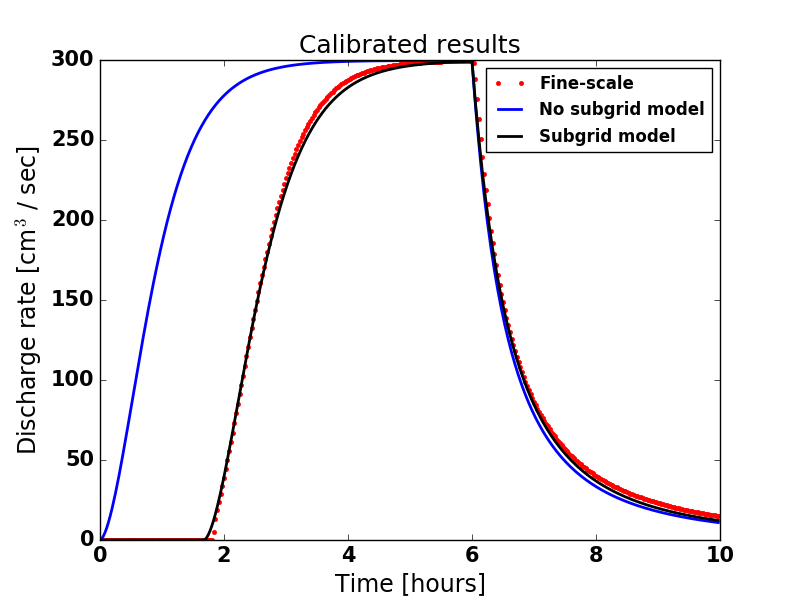
\includegraphics[width=6.2cm, height=5.5cm]{./figures/POLYGON_B01/POLYGON_B01dischargeCalibDDManning.png}
\includegraphics[width=6.2cm, height=5.5cm]{./figures/POLYGON_B01/POLYGON_B01watercontentCalibDDManning.png}
\caption{(Polygon B01) Comparison of the numerical results of the subgrid model with the fine-scale and without subgrid model results. Middle row: Calibrated value of the depression depth. Bottom row: Calibrated value of the depression depth and the manning coefficient.}
\label{polygon-B01}
\end{figure}


\section{Conclusions}\label{conclusion}

\section*{References}

\bibliography{reference}

\end{document}



